\section*{Introduction}

In \proj we propose to close the observe-assimilate-predict-sample
loop in the coastal ocean. Model skill, especially in the coastal ocean,
is highly dependent on poorly sampled in-situ measurements and remote
sensing data (when an overpass of a platform with appropriate sensors
is available to observe dynamic phenomenon). Typically ship-board
measurements, augmented by some fixed assets such as buoys, or
Lagrangian floats constitute the bulk of the observations. Quite often
these are not assimilated or if so, then frequently leading to poor
predictive skill. Our objective is to demonstrate the applicability of
adaptively controlled marine robots in the aerial, surface and
underwater domains, being able to sample the upper water-column 'at
the right place and time' driven by ocean models with increasing
predictive skill. Fig. \ref{fig:block-diag} shows a conceptual view of
the proposed field experiment.

\begin{figure}[!b]
  \centering
  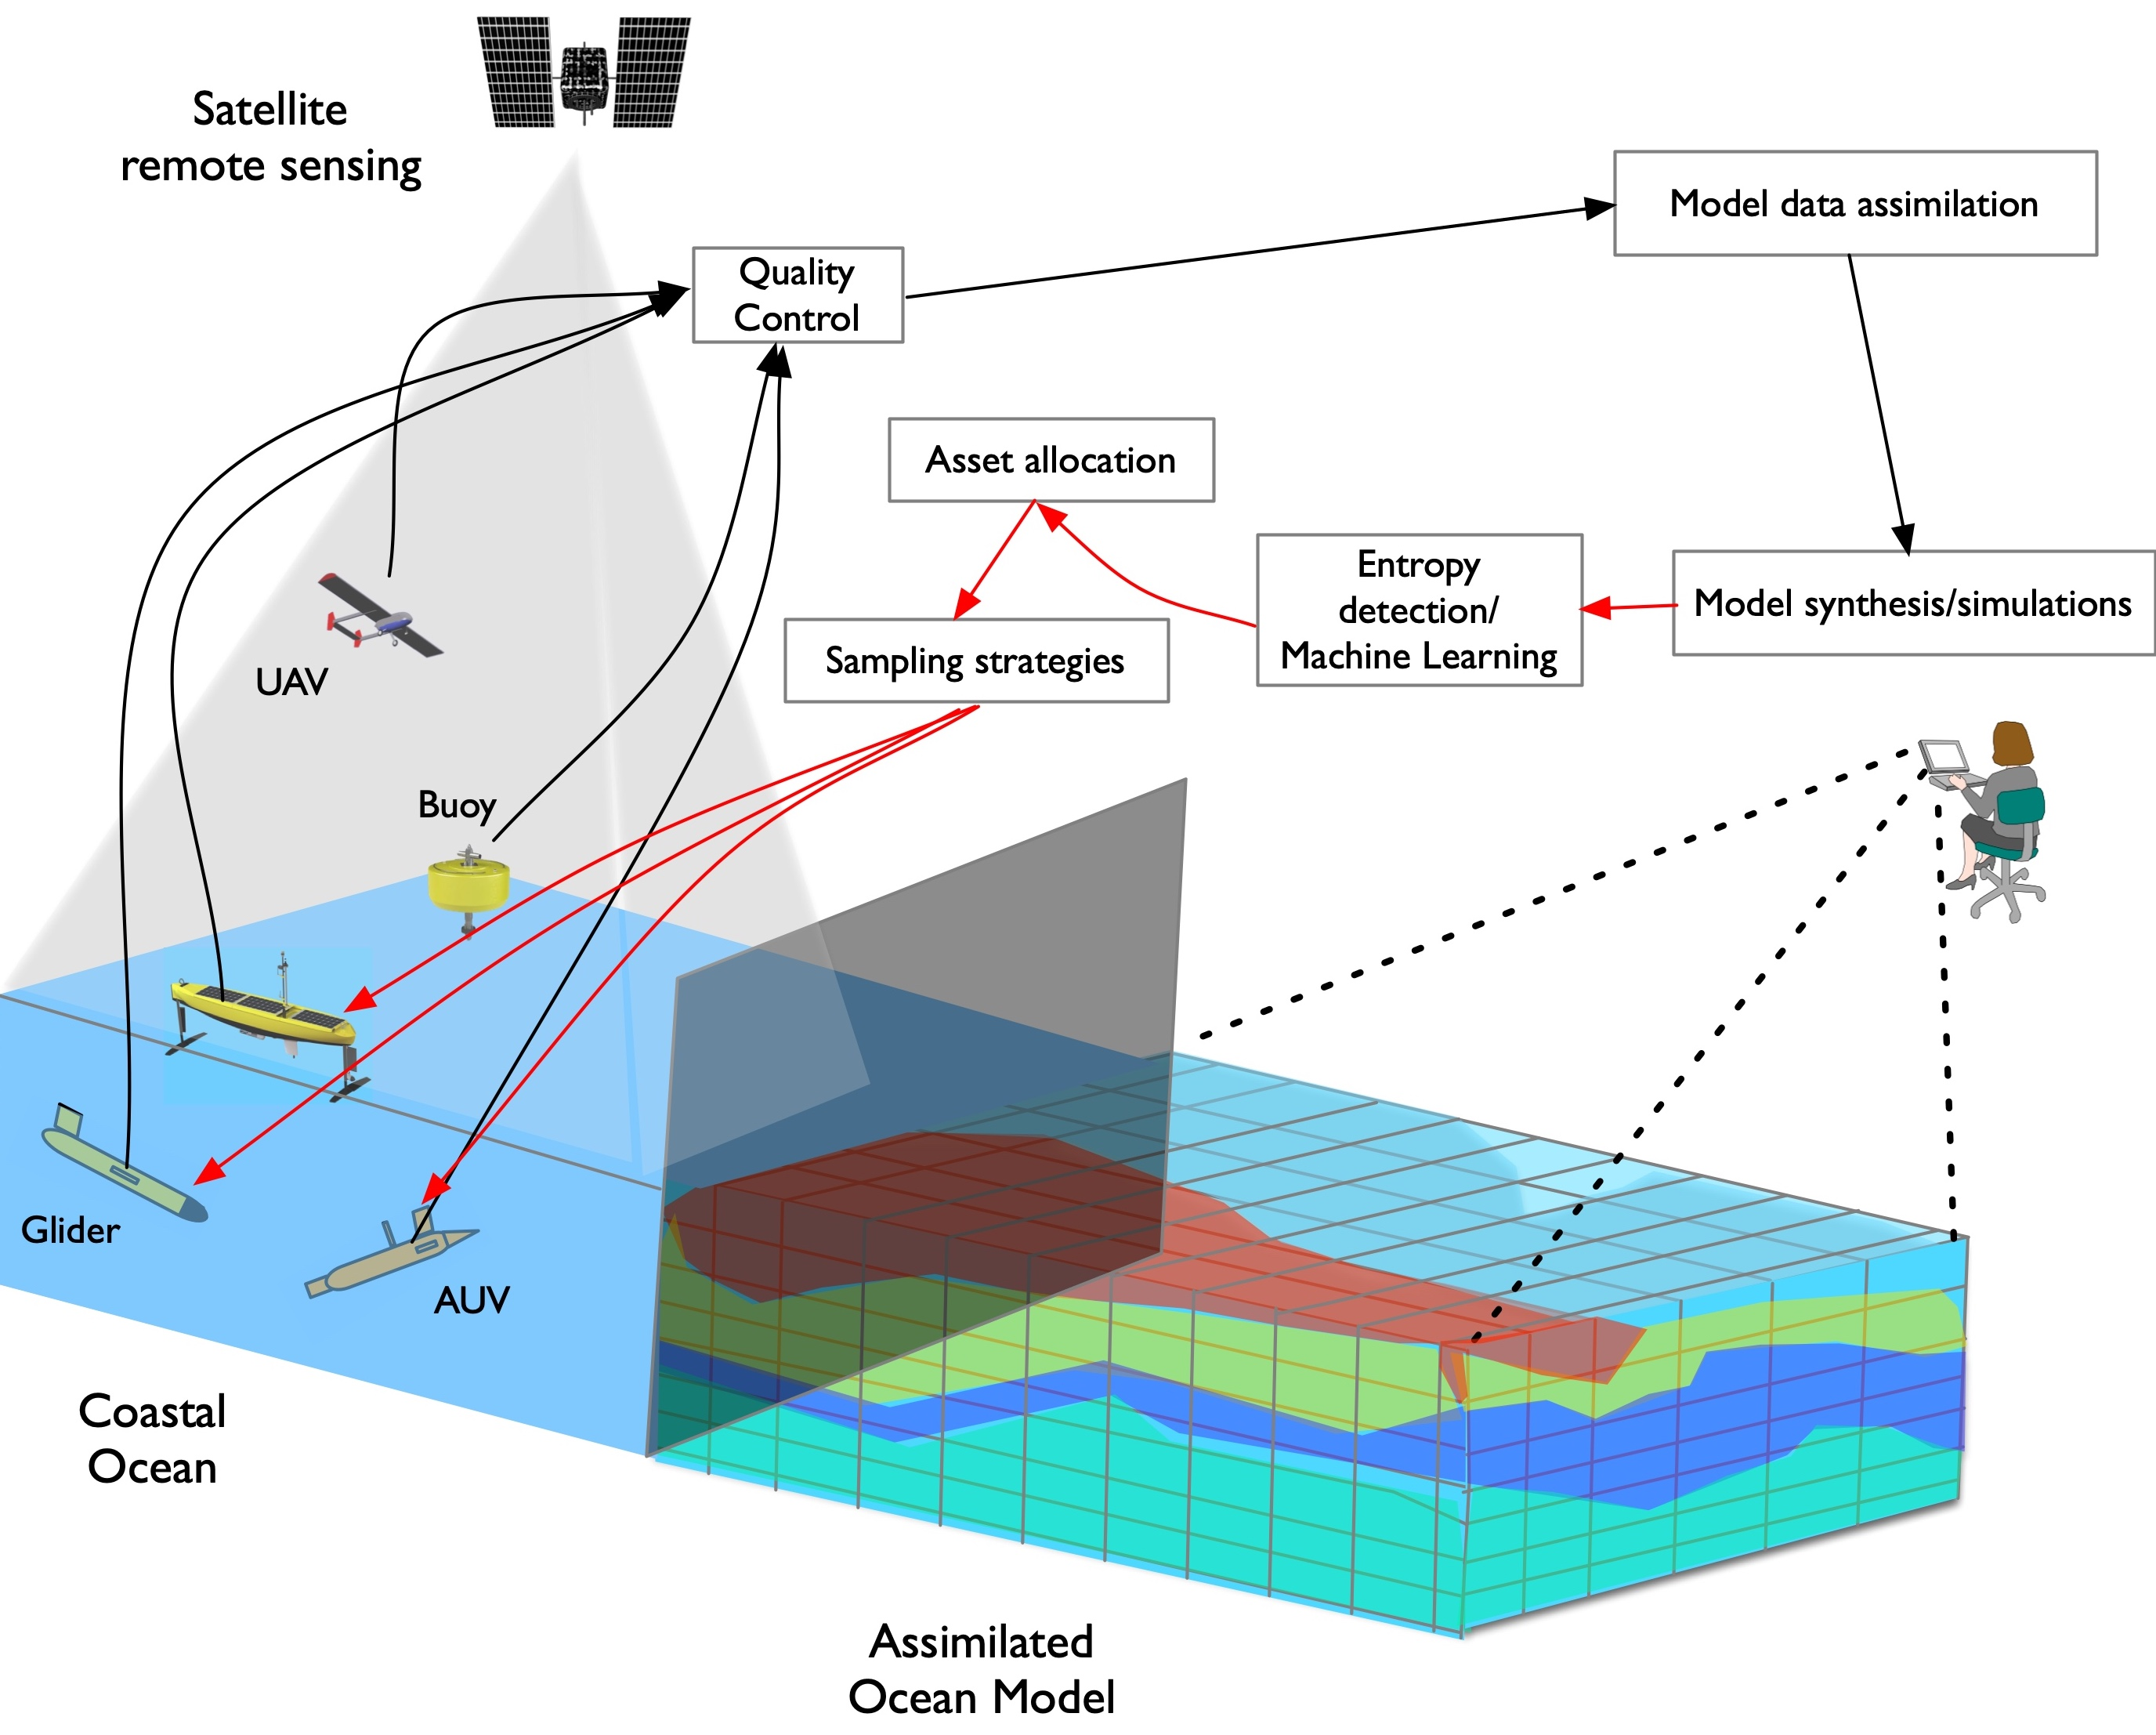
\includegraphics[scale=0.15]{fig/ensemble.jpg}
  \caption{\proj will integrate ocean models with adaptive robotic vehicles
    in the coastal ocean, to increase model skill while increasing
    model accuracy and prediction with a tight loop.}
  \label{fig:block-diag}
\end{figure}

\section*{Motivation}

\proj in an inter-disciplinary field driven experiment with a range of
motivations across science and engineering and spanning the fields of
Physical and Biological Oceanography, Artificial Intelligence
(including Machine Learning), autonomous systems and Spatial
Statistics. It will bring together researchers from these diverse
fields (all of whom have worked with one another) to build on the
integrative aspects of ocean observation especially in a dynamic
coastal environment.  In doing so, the tight integration between model
prediction and assimilation will be enhanced, so as to provide
realistic forecasts of a range of bio-physical variables including
temperature, salinity, wind, surface and sub-surface currents which will be used to intelligently drive sampling robots in the air, surface and
underwater. Important outcomes of this proposed project include:

\begin{itemize}[noitemsep,topsep=5pt,parsep=0pt,partopsep=0pt,leftmargin=0.5cm]

\item rapid assessment of environmental state using state of the art
  methods in modeling, control and sampling with minimal human intervention
\item increasing model prediction with targeted sampling
\item real-time decision support to determine appropriate mix of
  robotic or manned assets (e.g. small boats or research vessel) for
  targeted sampling
\item demonstration of coordinated observations with an ensemble of
  robotic vehicles
\end{itemize}

\section*{Location}

\begin{wrapfigure}{!h}{3.5in}
  \vspace{-0.5cm}
  \centering
  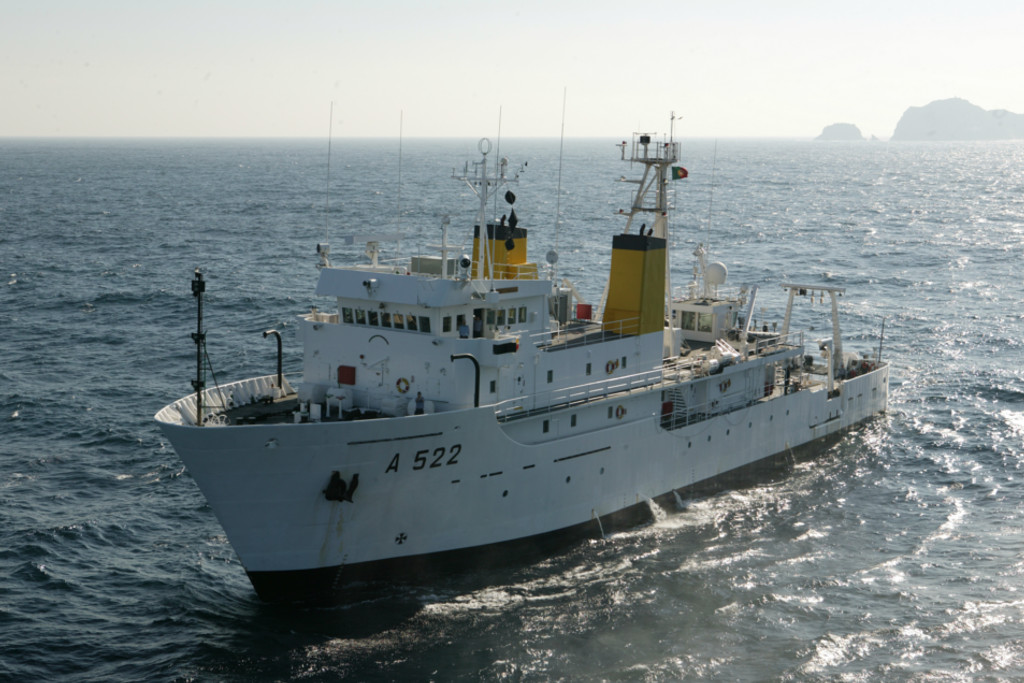
\includegraphics[scale=2]{fig/dom-carlos.jpg}
  \caption{A 70m research vessel, the NRP \emph{Dom Carlos} or its
    sister vessel will be available for 1 week for \proje.}
  \vspace{-0.3cm}
 \label{fig:vessel}
\end{wrapfigure}


We propose to hold the field experiment off of the coast of Portugal
near the town of Nazar\'e for a number of important reasons. The
region offers one of the deepest canyon's in continental Europe with
powerful tidal pumping, generation of internal waves, canyon driven
upwelling with filament dispersal along the south and the northern
coasts as well as into the Atlantic. The shallow shelf ($\sim 30--50$
meters) and the presence of two islands just offshore provide an
interesting range of bio-geo-physical phenomenon not observed
elsewhere including routine 30 meter waves in the surf zone; as a
result Nazar\'e is renowned as a surfing location
~\footnote{\url{https://www.youtube.com/watch?v=GJc4Ir78KdE}, and
  \url{https://www.youtube.com/watch?v=74pnrYPozcU}} with substantial
media coverage especially in the English speaking world.  Equally, the
Portuguese Hydrografic Institute
(\inste)~\footnote{\url{https://www.hidrografico.pt/}} maintains two
multi-parameter buoys as well as tide gauges in the vicinity of the
canyon. We propose to leverage their twice yearly maintenance visits
by their research vessels (Fig. \ref{fig:vessel}) to augment our
logistical support and therefore propose to hold the experiment in the
September-October 2021 timeframe. If planned in advance, the vessels
can be made available for \proj for a duration of 1 week. See
Fig. \ref{fig:studyarea-1} and \ref{fig:studyarea-2}.

\begin{figure}[!h]
  \vspace{-0.5cm} \centering \subfigure[Map of Portugal and the study
  area highlighted with the red
  rectangle.]{\label{fig:po-map}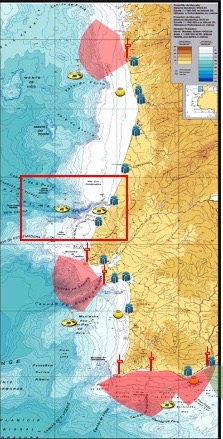
\includegraphics[scale=0.5]{fig/po-map.jpeg}}
  \hspace{+0.3cm} \subfigure[Zoomed in bathymetry showing the Nazar\'e
  canyon-Berlengas area (isobaths with depth in meters) and its
  environment including the placement of the two
  buoys.]{\label{fig:domain}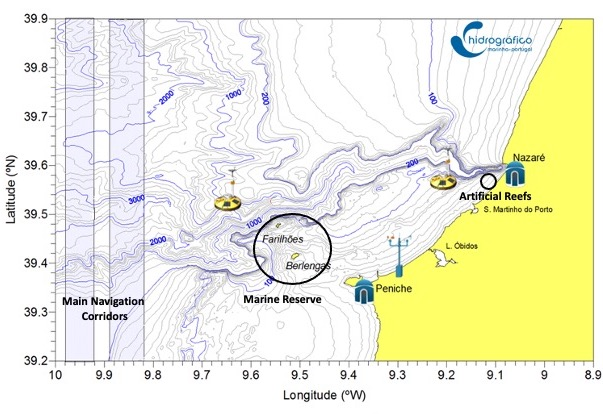
\includegraphics[scale=0.5]{fig/domain.jpg}}
  \subfigure[Predictions of currents and temperature at 10m depth from
  a \texttt{HOPS} (Harvard Ocean Prediction System) model with
  assimilation of temperature and salinity measurements collected by
  CTD profiles and
  current-meters.]{\label{fig:model}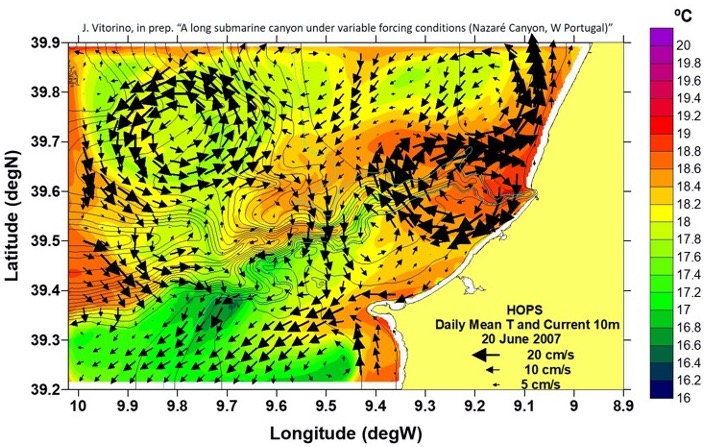
\includegraphics[scale=0.50]{fig/model.jpeg}}
  \caption{\subref{fig:po-map} \& \subref{fig:domain} show detailed
    views of the proposed study area for \proje, while
    \subref{fig:model} shows model predictions for the dynamic region
    driven by bathymetry and external forcing.}
  \label{fig:studyarea-1}
\end{figure}


\begin{figure}[!h]
  \vspace{-0.5cm}
  \centering
  \subfigure[]{\label{fig:chlshelf}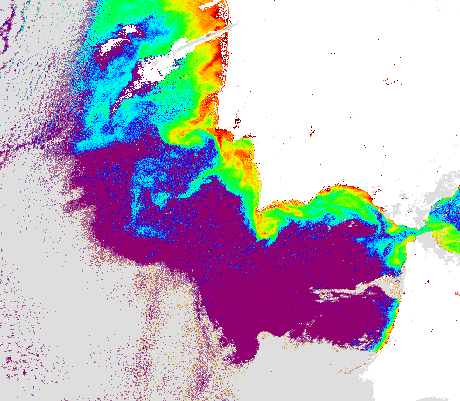
\includegraphics[scale=0.45]{fig/chl-shelf.png}}
  \subfigure[]{\label{fig:chldomain}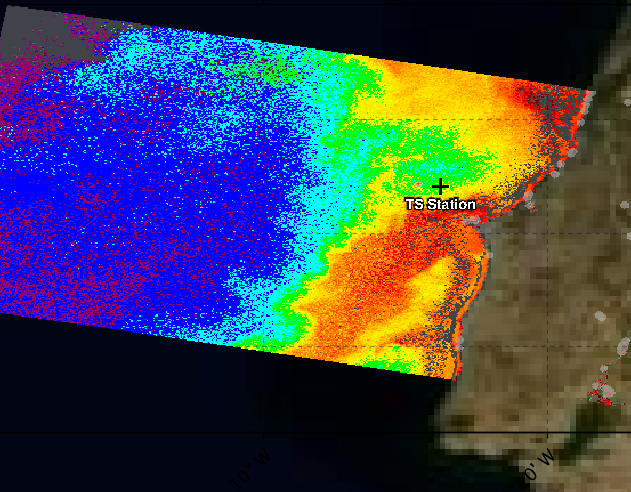
\includegraphics[scale=0.4]{fig/chl-domain.png}}
  \subfigure{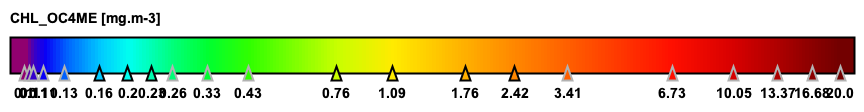
\includegraphics[scale=0.3]{fig/legend.png}}
  % \hspace{+0.3cm} 
  \subfigure[]{\label{fig:tmpchange}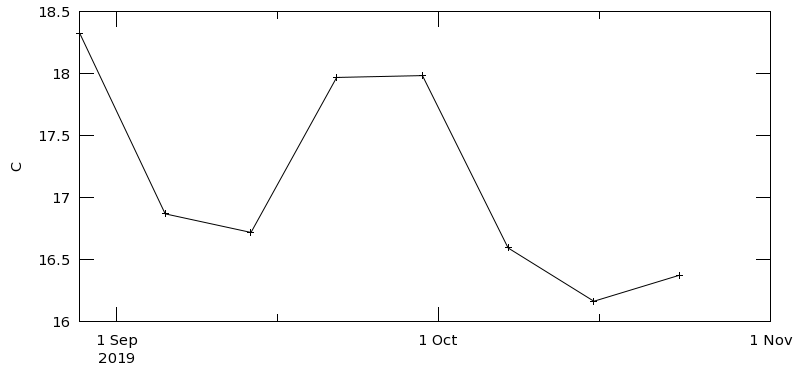
\includegraphics[scale=0.285]{fig/temp-change.png}}
  \subfigure[]{\label{fig:chlchange}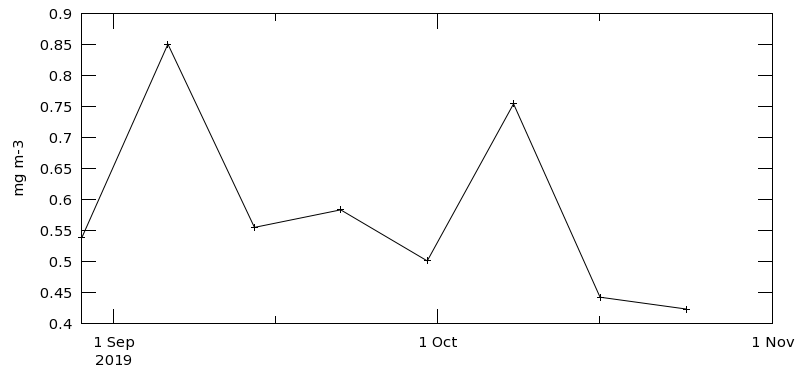
\includegraphics[scale=0.285]{fig/chl-change.png}}
  \caption{300m resolution remote sensing images from Sentinel 3 from
    September 6\textsuperscript{th} 2019 showing along shelf
    \subref{fig:chlshelf} and zoomed in Chlrophyll filaments
    \subref{fig:chldomain} emanating from the proposed study area of
    Nazar\'e canyon-Berlengas. \subref{fig:tmpchange} and
    \subref{fig:chlchange} show time series with rapid changes of
    temperature and chlorophyll respectively in the area.}
  \label{fig:studyarea-2}
\end{figure}

\section*{Logistical and budgetary information}

Off shore in the Nazar\'e canyon-Berlengas area are two islands of
Berlengas and Farilho\~es part of a protected nature preserve. With
special permission we expect to be able to be based in Berlengas for a
period of 3 weeks to conduct off shore operations. A small team will
also be present onboard the \inst research vessel where deployment and
recovery of assets need to be done well off shore at the boundaries of
the survey region. In addition \inst will be in a position to provide
a RHIB or a rigid boat for near-shore operations from the two
islands.

\univ will provide the bulk of the robotic assets including
aerial, surface and underwater vehicles as also the team to operate
them. The team will be split between being based in Berlengas, the
research vessel and also provide remote monitoring from Porto. \soc
will provide at least one glider to operate outside the shelf to
augment model observations in the meso-scale.

Our approximate leveraged budget for this exercise is expected to be
$\sim \$100$ K to support this 21 day (3 week) operation. This
includes all robotic vehicles, the ship time and personnel from
\inste, faculty and staff from all the partner organizations,
transportation of assets and people in Portugal as also insurance and
communication costs for and during the exercise. The budget will
support software development to extend observation quality control,
assimilation and ML based approaches to entropy reduction in modeling.

\paragraph{Roles and responsibilities} \univ will be the lead
organization, provide aerial, surface and underwater vehicles,
communication equipment and command/control software while
coordinating all activities. Funding requested will primarily support
students and staff in Porto for software development and
operations. \inst will provide the assimilation, modeling and
prediction with shore-side models. In addition \inst will provide
access to their research vessel as well as a RHIB or rigid boat. \mit
will support \inst for \texttt{HOPS} modeling and augmentation for ML
capabilities within. \colo and \ave will work on making biological
measurements and providing analysis and data to augment \inst
modeling. Table \ref{tab:roles} summarizes the roles and contributions
of all partners.

\begin{table}[!t]
  \centering
  \vspace{-0.5cm}
  \begin{tabular}{|p{1.5cm}|p{8cm}|p{6cm}|}\hline 
    \rowcolor{Gray}
    \bfseries Inst. &\bfseries Role &\bfseries Contributions\\
    \hline
    \org & Co-Lead organization, reporting, experiment design, outreach&\\
    \hline
    \univ & Co-Lead organization, CONOPS (concept of ops) design and
            implementation, software engineering
                                    &aerial/surface/underwater
                                      vehicles, comms,operations team\\
    \hline
    \inst & Physical Oceanography, Modeling, observation assimilation, prediction&\inst
                                                            research
                                                            vessel and
                                                            RHIB/rigid
                                                            boats,
                                                            local outreach\\
    \hline
    \ave & Biological sampling, lab analysis&\\
    \hline
    \soc & Physical Oceanography, glider operations& Gliders\\
    \hline
    \colo & Biological Oceanpgraphy, sampling&\\
    \hline
    \mit & Modeling, Machine Learning and entropy reduction&\\
    \hline
  \end{tabular}
  \caption{Roles and responsibilities and in-kind contributions in
    \proj for the 2021 Sept-Oct field experiment. All team members
    will be involved in experiment design and publishing post experiment.}
  \label{tab:roles}
\end{table}

\paragraph{Operational Considerations} While most experiments in the
coastal zone rely on ship-board measurements and gliders, the
challenging nature of this high-energy environment requires a mix of
assets in addition to gliders. Currents can be in the region of
$\sim 2$ knots, there is substantial variability in the upper
water-column and with high primary productivity and the existence of
coastal upwelling to provide for a rich nutrient base, the region has
a robust presence of fishermen, nets and crab pots. We expect to field
an ensemble of low cost robotic vehicles including propeller driven
AUVs, unmanned surface vehicles and aerial vehicles with RGB and
potentially hyper-spectral imaging sensors. Accessibility to the two
islands will also provide some shelter from weather for continuous
operations including rapid launch/recovery of in-situ assets. In
addition, the PIs are in negotiations with \nas for one or more
overpasses of the \textbf{SeaHawk} nano-satellite with a
hyper-spectral
imager~\footnote{\url{https://uncw.edu/socon/index.html}}. Finally,
\univ and \inst have a number of low cost temperature/density sensors
which when calibrated with CTDs on the vessel and robotic vehicles,
will enable local fisherman to provide timely data in this large
meso-scale region. All such data will be assimilated into the ocean
models run by \inst and supported by \univ2 which continues to support
\texttt{HOPS} development.

\paragraph{COVID protocol} As per standard oceanographic cruise
protocol in current circumstances, we will follow the guidance of WHO
and the US CDC; all personnel will isolate 5 days before the
experiment after appropriate PCR tests for safety and stay in one
pod. Those onboard the \inst research vessel will follow Portuguese
Navy guidelines and also isolate prior to the cruise and have no
contact with shore based personnel during the course of the
experiment.

\section*{Outreach}

\inst has had continued and extensive engagement over the years with
the local authorities including the Nazar\'e city officials and local
fishermen. As a result we believe in engaging fishermen to carry our
low cost temperature/density sensors and also help provide access to
the team to be able to commute to the islands when necessary, subject
to health protocols. In addition, we expect to engage local high
school students prior and after the experiment, to entice them into
thinking about careers in science and technology, much as we have done
in the past with success in another ONR funded
program~\footnote{\url{https://sunfish.lsts.pt/en/outreach/education}}.

With the world-wide interest in the area \proj will also work with the
local authorities and \inst to showcase our work in Portuguese and
English language media outlets.

Finally, publications resulting from the project will be targeted
towards peer-reviewed journals including \emph{Science Robotics,
  J. Field Robotics, Int. J. of Robotics Research, AI Journal,
  Autonomous Robots, Oceanography, PLOSone, Frontiers} and high-impact
conferences such as \emph{AAAI, IJCAI, ISER, ICAPS, RSS, IROS, ICRA
  and IEEE AUV} where we have frequently published.

